%%%%%%%%%%%%%%%%%%%%%%%%%%%%%%%%%%%%%%%%%
% Thin Sectioned Essay
% LaTeX Template
% Version 1.0 (3/8/13)
%
% This template has been downloaded from:
% http://www.LaTeXTemplates.com
%
% Original Author:
% Nicolas Diaz (nsdiaz@uc.cl) with extensive modifications by:
% Vel (vel@latextemplates.com)
%
% License:
% CC BY-NC-SA 3.0 (http://creativecommons.org/licenses/by-nc-sa/3.0/)
%
%%%%%%%%%%%%%%%%%%%%%%%%%%%%%%%%%%%%%%%%%

%----------------------------------------------------------------------------------------
%	PACKAGES AND OTHER DOCUMENT CONFIGURATIONS
%----------------------------------------------------------------------------------------

\documentclass[a4paper, 11pt]{article} % Font size (can be 10pt, 11pt or 12pt) and paper size (remove a4paper for US letter paper)

\usepackage[protrusion=true,expansion=true]{microtype} % Better typography
\usepackage{graphicx} % Required for including pictures
\usepackage{wrapfig} % Allows in-line images
\usepackage{float}
\usepackage{mathpazo} % Use the Palatino font
\usepackage[T1]{fontenc} % Required for accented characters
\linespread{1.05} % Change line spacing here, Palatino benefits from a slight increase by default

\makeatletter
\renewcommand\@biblabel[1]{\textbf{#1.}} % Change the square brackets for each bibliography item from '[1]' to '1.'
\renewcommand{\@listI}{\itemsep=0pt} % Reduce the space between items in the itemize and enumerate environments and the bibliography

\renewcommand{\maketitle}{ % Customize the title - do not edit title and author name here, see the TITLE block below
\begin{flushright} % Right align
{\LARGE\@title} % Increase the font size of the title

\vspace{50pt} % Some vertical space between the title and author name

{\large\@author} % Author name
\\\@date % Date

\vspace{40pt} % Some vertical space between the author block and abstract
\end{flushright}
}

%----------------------------------------------------------------------------------------
%	TITLE
%----------------------------------------------------------------------------------------

\title{\textbf{Detecting Malware in Android Applications}\\ % Title
} % Subtitle

\author{\textsc{Jake Pitkin} % Author
\\{\textit{CS 6350 - Machine Learning}}} % Institution

\date{\today} % Date

%----------------------------------------------------------------------------------------

\begin{document}

\maketitle % Print the title section

%----------------------------------------------------------------------------------------
%	ABSTRACT AND KEYWORDS
%----------------------------------------------------------------------------------------

%\renewcommand{\abstractname}{Summary} % Uncomment to change the name of the abstract to something else


%----------------------------------------------------------------------------------------
%	ESSAY BODY
%----------------------------------------------------------------------------------------
\section*{Introduction}

The Android platform is the most popular mobile platform, holding nearly $85\%$ of the global smartphone marketshare. [1] Most of the available software for Android devices comes from public application markets such as Google Play or the Apple App Store. As a result, Android users are a popular target for malicious software. 

The goal is to classify software as malicious or not as a way to improve the security of the Android platform. This will be accomplished by training a classifier on examples where we observed how often particular system calls were called. The hope is this will expose a patterns of system calls that malicious applications make. Allowing us to prohibit these applications from public markets and protect users.
 
%------------------------------------------------

\section*{Approach - Random Forest}
The approach I used to classify the maliciousness of an Android application is a random forest. A random forest is an ensemble method based on bagging (short for bootstrap aggregating) and decision trees using the ID3 algorithm. In the classic ID3 algorithm, all features are considered (using the heuristic of information gain to select a feature at each level) and one tree is trained on all the training examples. In a random forest, \textit{N} decision trees are trained. For each tree, I randomly selected \textit{m} examples with replacement and only consider \textit{k} random features when building the tree.

When it came time to predict a label for a new example, all of the trees in the random forest vote on the label. As I was performing binary classification, I chose $N$ to be odd and took the majority vote of the trees.

\begin{figure} [H]
  \centerline{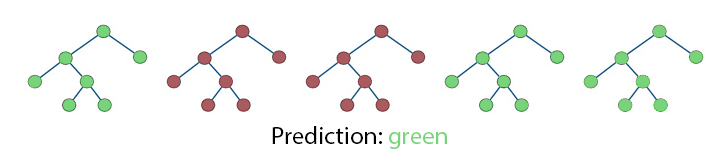
\includegraphics[width=0.8\linewidth]{decision_tree.png}}
  \caption{Taking the majority vote of an ensemble of decision trees.}
\end{figure}

\section*{Feature Exploration}

Each example is defined by 360 features or system calls. But I discovered only 130 of these features appear in the training examples. Of these 130 features, there are a great deal of them that appear in nearly every training example and four features appear in every training example. The 65 features with the highest frequency appear in at least half of the training examples.

A feature's value is defined by how many times the system call that feature represents is called. As such, the range of values a feature held varied greatly. Some present system calls occurred only a few times where others were called hundreds of thousands of times.

A decision tree classifier is only feasible with numeric feature values by using thresholds or by making the values discrete. I choose to make them discrete by transforming all features into either a $0$ or a $1$. I calculated the average value a feature held across all the training examples. I considered a feature to be "present" or $1$ if it's value is above the average and $0$ otherwise. I played with this threshold by introducing a hyper-parameter $\lambda$.

$$threshold_j = \lambda * average_j$$

This allowed me to vary how above-or-below the average a feature $j$ should be to be considered "present".

\section*{Cross-validation}
My random forest classifier contained four hyper-parameters, all of which were determined by using 6-fold cross validation.

\begin{table}[H]
{\renewcommand{\arraystretch}{1.2}%
\begin{tabular}{| c | c | c |}
\hline
Hyper-parameter & Description & Best Value\\
\hline
$\lambda$ & Decision boundary for discretization. & 0.34\\ \hline
N & Decision tree count. & 101\\ \hline
m & Size of training example sample. & 10,000\\ \hline
k & Number of randomly selected features. & 50\\ \hline
\end{tabular}}
\caption{The used hyper-parameters for the random forest classifier.}
\end{table}

If a system call was called at least 0.34 times the average, that feature was considered present an was given a value of $1$ and a value of $0$ otherwise. 

My random forest classifier consisted of $101$ decision trees. Each decision trees was constructed with 50 randomly selected features and was trained on 10,0000 sampled with replacement training examples.

\section*{Performance}
To determine the performance of my tuned random forest classifier, I considered its accuracy and F1 score on the training and test sets. I was happy with the margin between the classifier's accuracy on the training and test set being small. I found this to be a strength of using an ensemble as it generalized well.

\begin{table}[H]
{\renewcommand{\arraystretch}{1.2}%
\begin{tabular}{| c | c | c |}
\hline
Data Set & Accuracy & F1 Score\\
\hline
Training Set & 0.881 & 0.73\\ \hline
Test Set & 0.851 & 0.741\\ \hline
\end{tabular}}
\end{table}

At the time of this report I am currently $9th$ out of $28th$ on the Kaggle competition board with a score of $0.82819$.

\section*{Improvements}

\textit{Decision boundaries - }An area I would of liked to explore deeper was the discretization of the data. I took a fairly naive approach of using the average value of a feature as the boundary for transforming continuous features values into binary features. Being more analytical by looking at the distribution of labels relative to each feature value could have proven fruitful. Additionally, rather than making all features binary, using multiple decision boundaries to have a handful of possible feature values could of been worthwhile.

\bigbreak
\noindent
\textit{SVM on random forest votes - } My random forest classifier used a majority vote between all the trees to decide on a final label. I would of liked to train a SVM classifier using these predictions as features (as we explored in homework 4).

\section*{Other Classifiers Attempted}

I tried many other classifiers before arriving at using a random forest. Other than decision trees, I tried different classifiers with transformed features and unmodified features. Here is how they each ranked according to their performance on the Kaggle submission data. 

\begin{enumerate}
	\item Logistic regression with binary features
	\item Logistic regression
	\item Decision tree with binary features
	\item SVM with binary features
	\item Margin perceptron
	\item Aggressive margin perceptron
	\item Perceptron
\end{enumerate}

With my final classifier, a random Forest, out performing all of the above classifiers. Logistic Regression with binary features was a very close second with performance within a percent of a random forest.

\section*{Evolution of My Project}

My project began by taking the naive approach of applying a linear classifier on the dataset as is. I discovered there were many irrelevant features and each feature could take a wide range of values. To remedy this, I only used relevant features and discretized the feature values. Ultimately, I moved away from a linear classifier to an ensemble of decision trees. I initially tried a random forest as the winner of the Netflix challenge discussed in class used an ensemble method. When I saw results that were generalizing well I stuck with it and began to tune the hyperparameters.

\section*{What I Would Like To Try}

I wish I would of had time to implement a neural network this semester. They are all the hype right now and from my limited knowledge seem to be creeping into all fields of AI. My intention is to find a fun problem over winter break and try to solve it with a neural network.

Another skill I would like to improve is visualizing and exploring datasets. I would of liked to have better tools and exploring the feature set so I could of made smarter decisions about determining which features were relevant and how to discretize their feature values.

\section*{What I Learned}

I have learned so much in this course and I know I am barely scratching the surface. I entered the course with only a vague understanding of machine learning based on assumptions and news stories I came by. Leaving the course I have a new appreciation for how much creativity is possible while being deeply mathematical at the same time.

I learned that theory is indispensable and helps formulate what is possible. And at the same time that the real world is messy and there is a lot of trial, error, and creativity in creating solid systems. I saw that AI is quite often romanticized by the media and misunderstood as magic by many. I find it really enjoyable exploring the limitations of these technologies and understanding how they work to dispel these myths. 

Your course, along with Prof. Riloff's NLP course, has piqued my interest in furthering my education and I am now considering PhD programs after finishing my MS. Next semester I will be taking Structured Prediction, Theory of Machine Learning, and Information Extraction to dive in deeper. My hope is to find a sub-field of machine learning that  resonates with me.

I want to thank you for a fantastic course and I really look forward to next semester.
\section*{References}
[1] Dimja\v{s}evi\'{c}, M., Atzeni, S., Ugrina, I. and Rakamaric, Z., 2016, March. Evaluation of Android Malware Detection Based on System Calls. In Proceedings of the 2016 ACM on International Workshop on Security And Privacy Analytics (pp. 1-8). ACM.

\end{document}